%!TEX program = lualatex
%!TEX encoding = UTF-8 Unicode  
%!TEX root = chapter09.tex  
\documentclass[main.tex]{subfiles}
\begin{document} 
%----------------------------------------------------------------------------------------
%	CHAPTER 09
%----------------------------------------------------------------------------------------
\cleardoublepage
\loadgeometry{marginlayout}  
\pagestyle{scrheadings} % Print headers again  
\KOMAoptions{
	headwidth=textwithmarginpar,
	headsepline=true,
	headsepline= 0.5pt,
	footwidth=textwithmarginpar,
}   
\onehalfspacing 
\setcounter{chapter}{8}

\chapter{Fonctions de référence (1) : fonction carré et racine carrée}
 

\noindent Dans l'étude d'une fonction ou d'une classe de fonctions on doit savoir :
\begin{enumerate}[leftmargin=*,label=\arabic*)]
	\item calculer l'image/l'ordonnée $y=f(x)$ d'une abscisse donnée.
	\item connaitre le sens de variation de $f$ et dresser son tableau de variation.
	\item Pour $k\in\mathbb{R}$, connaitre le nombre de solutions de l'équation $f(x)=k$ inconnue $x$, et la résoudre. 
	En particulier résoudre $f(x)=0$
	\item Pour $k\in\mathbb{R}$, savoir résoudre l'inéquation $f(x)\geqslant k$ inconnue $x$.\\
	En particulier dresser son tableau de signe.
	\item connaitre les propriétés de sa représentation graphique.  
\end{enumerate}
\vspace{-1em}
%----------------------------------------------------------------------------------------
%	 
%----------------------------------------------------------------------------------------
\newpage 
\loadgeometry{marginlayout}  
\pagestyle{scrheadings} % Print headers again  
\KOMAoptions{
	headwidth=textwithmarginpar,
	headsepline=true,
	headsepline= 0.5pt,
	footwidth=textwithmarginpar,
}   
\onehalfspacing  


\section{Fonction carré}   
\begin{definition}
	La fonction carré est  la fonction définie sur $\mathbb{R} $ par $f(x)=x^2$ 
\end{definition}
Un carré est toujours positif ou nul : pour tout $x\in\mathbb{R}$ on a $x^2 \geqslant 0$.
\begin{proposition}[sens de variation]  
	La fonction carré  est strictement décroissante sur $\interval[open left]{-\infty}{0}$  et strictement croissante sur  $\interval[open right]{0}{-\infty}$ :  
	\begin{enumerate}[label=\textbullet]
		\item  Si $a<b\leqslant 0$ alors $a^2>b^2\geqslant 0$
		\item Si $0\leqslant  a<b$ alors $0\leqslant   a^2<b^2$
	\end{enumerate}
\end{proposition}
\begin{figure}[h]
	\begin{tikzpicture}
		%\tikzset{  double style/.style = {double,very thick,double distance=2pt}}
		\tikzset{  double style/.style = {double,thick,double distance=2pt}}
		\tkzTabInit[lgt = 3.5, espcl =3.5, color, colorC = blue!15, colorL = green!15]{$x$ / 1 ,$f(x)=x^2$ / 1.5,  Signe de $f(x)$/ 1.0  }{$-\infty$ ,$0$ , $+\infty$} 
		\tkzTabVar{+/$+\infty$  ,- /$0$,  +/ $+\infty$} 
		\tkzTabLine{,+,z,+,}% 
	\end{tikzpicture}  
	\caption{Tableau de variation de la fonction carré} 
\end{figure} 
\begin{proof}\emph{Exigible en fin de seconde}\hfill 
	\vfill 
\end{proof}  
\begin{figure}[!ht]
	\begin{tikzpicture}[xscale=0.75, yscale=0.75]
		\tkzSetUpPoint[size=3, fill=black]
		\tkzfctset{tan style/.style={->,>=latex, color=red, line width=1.2pt}}  
		\tkzInit[xmin=-6,xmax=6,ymin=-1,ymax=8,xstep=1.0, ystep=1.0];
		\begin{scope}[dashed] 
			\tkzGrid[color=gray, line width=0.5pt]
		\end{scope}  
		\tkzDrawX[  noticks, font=\scriptsize, line width=2pt, label=$x$, above =10pt  ] 
		\tkzDrawY[  noticks,  font=\scriptsize, line width=2pt , label={$y$}, right=5pt ]  
		\tkzLabelXY[orig = false,  font=\scriptsize]
		\tkzRep[color  = Maroon,line width = 2pt, posxlabel=below, posylabel=left, xnorm=1, ynorm=1] 
		\tkzFct[domain = -5.0:4.0, line width=2pt,samples=100,color = red]{(\x**2)} 
		\tkzFct[domain = -2.0:6.0, line width=1.2pt,dashed, samples=2]{(\x)} 
		
		\tkzDefPoint(3,8){P} 
		\tkzDefPoint(5,4){Q} 
		\tkzText[color = black, below right  , fill=white](P){$\mathcal{P}\colon y=x^2$}
		\tkzText[color = black, above , fill=white](Q){$y=x$}
		\tkzPointShowCoord[ color=blue, line width=1.2pt  ](1,1) \tkzPointShowCoord[  color=blue, line width=1.2pt ](-1,1) 
	\end{tikzpicture}
	\caption{La courbe représentative de la fonction carré est la \textbf{parabole}  d'équation $\mathscr{P}\colon y=x^2$.}
\end{figure}


%----------------------------------------------------------------------------------------
%	 
%---------------------------------------------------------------------------------------- 
\newpage 
\loadgeometry{widelayout}  
\pagestyle{scrheadings} % Print headers again  
\KOMAoptions{
	headwidth=textwithmarginpar,
	headsepline=true,
	headsepline= 0.5pt,
	footwidth=textwithmarginpar,
} 
\onehalfspacing
\begin{figure*}[!ht]
	\begin{minipage}{0.3\linewidth}\centering
		\fbox{$k<0$} \\
		\begin{tikzpicture}[scale=1.0]
			\tkzSetUpPoint[size=5, fill=black]
			\tkzfctset{tan style/.style={->,>=latex, color=red, line width=1.2pt}}  
			\tkzInit[xmin=-2.1,xmax=2.1,ymin=-1.5,ymax=3.5,xstep=1, ystep=1];
			\tkzFct[domain = -3:3,  line width=2.0pt, color=red]{\x**2}  
			\tkzDefPoint(0,-0.8){Q3}
			\tkzLabelPoint[below right](Q3){$k$}
			\tkzDrawXY[noticks,  font=\scriptsize, line width=2pt ]%[orig=false] 
			\tkzText[below left ](0,0){$O$};  
			\tkzHLine[color = blue , line width= 1.2pt, dashed, label=$y=k$]{-0.9}
			\tkzRep[color  = Maroon,line width = 2pt, posxlabel=below, posylabel=left, xnorm=1, ynorm=1] 
		\end{tikzpicture}\\
		pas de solution $S=\emptyset$
	\end{minipage} 
	%\hfill 
	\begin{minipage}{0.3\linewidth}\centering
		\fbox{$k=0$} \\
		\begin{tikzpicture}[scale=1.0]
			\tkzSetUpPoint[size=5, fill=black]
			\tkzfctset{tan style/.style={->,>=latex, color=red, line width=1.2pt}}  
			\tkzInit[xmin=-2.5,xmax=2.1,ymin=-1.5,ymax=3.5,xstep=1, ystep=1];
			\tkzFct[domain = -3:3,  line width=2.0pt, color=red]{\x**2} 
			\tkzDefPointByFct(0) \tkzGetPoint{P1}  \tkzDrawPoints(P1) 
			\tkzDrawXY[noticks,  font=\scriptsize, line width=2pt ]%[orig=false] 
			\tkzText[below left ](0,0){$O$};  
			\tkzHLine[color = blue , line width= 1.2pt, dashed, label=$y=0$]{0}
			\tkzRep[color  = Maroon,line width = 2pt, posxlabel=below, posylabel=left, xnorm=1, ynorm=1] 
		\end{tikzpicture}\\
		solution unique $S=\{ 0\}$
	\end{minipage} 
	%\hfill
	\begin{minipage}{0.3\linewidth}\centering
		\fbox{$k>0$} \\
		\begin{tikzpicture}[scale=1.0]
			\tkzSetUpPoint[size=5, fill=black]
			\tkzfctset{tan style/.style={->,>=latex, color=red, line width=1.2pt}}  
			\tkzInit[xmin=-2.1,xmax=2.1,ymin=-1.5,ymax=3.5,xstep=1, ystep=1];
			\tkzFct[domain = -3:3,  line width=2.0pt, color=red]{\x**2} 
			\tkzDefPointByFct(1.5) \tkzGetPoint{P1}
			\tkzDefPointByFct(-1.5)\tkzGetPoint{P2}\tkzDrawPoints(P1,P2)
			\tkzPointShowCoord[noydraw](P1)
			\tkzPointShowCoord[noydraw](P2)
			\tkzDefPoint(1.5,0){Q1}
			\tkzDefPoint(-1.5,0){Q2}
			\tkzLabelPoint[below](Q1){\scriptsize$\sqrt{k}$}
			\tkzLabelPoint[below](Q2){\scriptsize$-\sqrt{k}$}
			\tkzDefPoint(0,2.25){Q3}
			\tkzLabelPoint[above right](Q3){$k$}
			\tkzDrawXY[noticks,  font=\scriptsize, line width=2pt ]%[orig=false] 
			\tkzText[below left ](0,0){$O$};  
			\tkzHLine[color = blue , line width= 1.2pt, dashed, label=$y=k$]{2.25}
			\tkzRep[color  = Maroon,line width = 2pt, posxlabel=below, posylabel=left, xnorm=1, ynorm=1] 
		\end{tikzpicture}\\
		2 solutions $S=\{-\sqrt{k}; \sqrt{k}\}$
	\end{minipage} 
	\caption{Les solutions de l'équation $x^2=k$ inconnue $x$, selon les valeurs de $k$.}
\end{figure*} 

\begin{figure*}[!ht]
	\noindent\begin{minipage}{0.3\columnwidth}\centering
		\fbox{$k<0$} \\
		\begin{tikzpicture}[scale=1.0]
			\tkzSetUpPoint[size=5, fill=black]
			\tkzfctset{tan style/.style={->,>=latex, color=red, line width=1.2pt}}  
			\tkzInit[xmin=-2.3,xmax=2.3,ymin=-1.5,ymax=3.5,xstep=1, ystep=1];
			\tkzFct[domain = -3:3,  line width=2.0pt, color=red]{\x**2}  
			\tkzDefPoint(0,-0.8){Q3}
			\tkzLabelPoint[below right](Q3){$k$}
			\tkzDrawXY[noticks,  font=\scriptsize, line width=2pt ]%[orig=false] 
			\tkzText[below left ](0,0){$O$};  
			\tkzHLine[color = blue , line width= 1.2pt, dashed, label=$y=k$]{-0.9}
			\tkzRep[color  = Maroon,line width = 2pt, posxlabel=below, posylabel=left, xnorm=1, ynorm=1] 
		\end{tikzpicture}\\
		L'inéquation $x^2\leqslant k$ n'a pas de solution : $S=\emptyset$
		
		L'inéquation $x^2\geqslant k$ est toujours vraie : $S=\mathbb{R}$
	\end{minipage}
	%\hfill
	\begin{minipage}{0.65\columnwidth}\centering
		\fbox{$k>0$} \\
		\begin{tikzpicture}[scale=1.0]
			\tkzSetUpPoint[size=5, fill=black]
			\tkzfctset{tan style/.style={->,>=latex, color=red, line width=1.2pt}}  
			\tkzInit[xmin=-2.3,xmax=2.3,ymin=-1.5,ymax=3.5,xstep=1, ystep=1];
			\tkzFct[domain = -3:3,  line width=2.0pt, color=red]{\x**2} 
			\tkzDefPointByFct(1.5) \tkzGetPoint{P1}
			\tkzDefPointByFct(-1.5)\tkzGetPoint{P2}\tkzDrawPoints(P1,P2)
			\tkzPointShowCoord[noydraw](P1)
			\tkzPointShowCoord[noydraw](P2)
			\tkzDefPoint(1.5,0){Q1}
			\tkzDefPoint(-1.5,0){Q2}
			\tkzLabelPoint[below](Q1){\scriptsize$\sqrt{k}$}
			\tkzLabelPoint[below](Q2){\scriptsize$-\sqrt{k}$}
			\tkzDefPoint(0,2.25){Q3}
			\tkzLabelPoint[above right](Q3){$k$}
			\tkzDrawXY[noticks,  font=\scriptsize, line width=2pt ]%[orig=false] 
			\tkzText[below left ](0,0){$O$};  
			\tkzHLine[color = blue , line width= 1.2pt, dashed, label=$y=k$]{2.25}
			\tkzRep[color  = Maroon,line width = 2pt, posxlabel=below, posylabel=left, xnorm=1, ynorm=1] 
		\end{tikzpicture}
		%  \hfill  
		\begin{tikzpicture}[scale=1.0]
			\tkzSetUpPoint[size=5, fill=black]
			\tkzfctset{tan style/.style={->,>=latex, color=red, line width=1.2pt}}  
			\tkzInit[xmin=-2.3,xmax=2.3,ymin=-1.5,ymax=3.5,xstep=1, ystep=1];
			\tkzFct[domain = -3:3,  line width=2.0pt, color=red]{\x**2} 
			\tkzDefPointByFct(1.5) \tkzGetPoint{P1}
			\tkzDefPointByFct(-1.5)\tkzGetPoint{P2}\tkzDrawPoints(P1,P2)
			\tkzPointShowCoord[noydraw](P1)
			\tkzPointShowCoord[noydraw](P2)
			\tkzDefPoint(1.5,0){Q1}
			\tkzDefPoint(-1.5,0){Q2}
			\tkzLabelPoint[below](Q1){\scriptsize$\sqrt{k}$}
			\tkzLabelPoint[below](Q2){\scriptsize$-\sqrt{k}$}
			\tkzDefPoint(0,2.25){Q3}
			\tkzLabelPoint[above right](Q3){$k$}
			\tkzDrawXY[noticks,  font=\scriptsize, line width=2pt ]%[orig=false] 
			\tkzText[below left ](0,0){$O$};  
			\tkzHLine[color = blue , line width= 1.2pt, dashed, label=$y=k$]{2.25}
			\tkzRep[color  = Maroon,line width = 2pt, posxlabel=below, posylabel=left, xnorm=1, ynorm=1] 
		\end{tikzpicture}\\
		L'inéquation $x^2\leqslant k$ a pour ensemble solution \\ $S=\interval{-\sqrt{k}}{\sqrt{k}}$
		
		L'inéquation $x^2\geqslant k$ a pour ensemble solution  $S=\interval[open left]{-\infty}{-\sqrt{k}}\cup \interval[open right]{\sqrt{k}}{+\infty}$
	\end{minipage}  
	\caption{Les solutions de l'inéquation $f(x)\leqslant k$ inconnue $x$.}
\end{figure*}
\begin{example}En isolant $x^2$, résoudre dans $\mathbb{R}$ les équations et inéquations suivantes d'inconnue $x$ :
	\begin{multicols}{4}
		\begin{enumerate}[label={\alph*)}, leftmargin=*] 
			\item $5x^2=15$ 
			\item  $x^2-5<11 $ 
			\item  $12>2x^2-2>7$ 
			\item $1-5x^2\geqslant 2$   
		\end{enumerate}
	\end{multicols}
\end{example}
%----------------------------------------------------------------------------------------
%	EXERCICES
%----------------------------------------------------------------------------------------

\newpage 
\loadgeometry{widelayout}  
\pagestyle{scrheadings} % Print headers again  
\KOMAoptions{
headwidth=textwithmarginpar,
headsepline=true,
headsepline= 0.5pt,
footwidth=textwithmarginpar,
} 
\onehalfspacing
\subsection{Exercices : fonction carré}
\begin{eBox}
Dans les exercices qui suivent, $f$ est la fonction carré définie dans $\mathbb{R}$ par $f (x) = x^2$ 
\end{eBox}
\vspace{-0.5em}
\begin{exercise}[calculer les images et antécédents par une fonction carré]\hfill   
\vspace{-0.5em}
%	\begin{multicols}{2}
\begin{spacing}{2} 
\begin{enumerate}[label={}, leftmargin=*]   
	\item  L'image de $-\sqrt{6}$ par la fonction $f$ est  \dotfill   
	\item $f(10^{-3})=$\dotfill $f\left(\frac{7}{13}\right)=$\dotfill $f(2\sqrt{3})=$\dotfill 
	\item Les antécédent de $10$ par $f$ sont \dotfill 
	\item La valeur \dotfill a un unique antécédent par la fonction $f$.
	\item Lorsque \dotfill alors l'équation $f(x)=k$ n'a pas de solutions. 
	\item $f(1-\sqrt{2})=$\dotfill 
	\item $f(x+1)=$\dotfill
\end{enumerate}
\end{spacing}
%\end{multicols}	
\vspace{-0.5em} 
\end{exercise}
\begin{example}[Utiliser le sens de variation de la fonction carré]\hfill \\
	Soit $a$ un nombre réel.  En s'aidant éventuellement de la courbe de la fonction carré ou de son tableau de variation, encadrer au mieux $a^2$ dans les cas suivants :
	
	\noindent\hfill\parbox{0.24\linewidth}{	
		$\begin{WithArrows}
			2\sqrt{3}&<a \leqslant 4 \\
			&  \rule{0pt}{1.8em} \\
			&  \rule{0pt}{1.8em}    
		\end{WithArrows}$ 	
	} \hfill\parbox{0.24\linewidth}{	
		$\begin{WithArrows}
			0 &<a<3 \rule{0pt}{1.8em} \\ % 
			&  \rule{0pt}{1.8em}  \\  
			&   \rule{0pt}{1.8em}    
		\end{WithArrows}$ 	
	} \hfill\parbox{0.31\linewidth}{	
		$\begin{WithArrows}
			-5&<a<3 \rule{0pt}{1.8em} \\ % 
			&  \rule{0pt}{1.8em}  \\  
			&   \rule{0pt}{1.8em}   
		\end{WithArrows}$ 	
	} 
\end{example} 
\begin{minipage}{0.3\linewidth}\centering 
	\begin{tikzpicture}[scale=1.0]
		\tkzSetUpPoint[size=5, fill=black]
		\tkzfctset{tan style/.style={->,>=latex, color=red, line width=1.2pt}}  
		\tkzInit[xmin=-2.1,xmax=2.1,ymin=-1.0,ymax=2.5,xstep=1, ystep=1];
		\tkzFct[domain = -3:3,  line width=2.0pt, color=red]{0.7*\x**2}  
%		\tkzDefPoint(0,-0.8){Q3}
%		\tkzLabelPoint[below right](Q3){$k$}
		\tkzDrawXY[noticks,  font=\scriptsize, line width=2pt ]%[orig=false] 
%		\tkzText[below left ](0,0){$O$};  
%		\tkzHLine[color = blue , line width= 1.2pt, dashed, label=$y=k$]{-0.9}
%		\tkzRep[color  = Maroon,line width = 2pt, posxlabel=below, posylabel=left, xnorm=1, ynorm=1] 
	\end{tikzpicture} 
\end{minipage} \hfill
\begin{minipage}{0.3\linewidth}\centering 
	\begin{tikzpicture}[scale=1.0]
		\tkzSetUpPoint[size=5, fill=black]
		\tkzfctset{tan style/.style={->,>=latex, color=red, line width=1.2pt}}  
		\tkzInit[xmin=-2.1,xmax=2.1,ymin=-1.0,ymax=2.5,xstep=1, ystep=1];
		\tkzFct[domain = -3:3,  line width=2.0pt, color=red]{0.7*\x**2}  
		%		\tkzDefPoint(0,-0.8){Q3}
		%		\tkzLabelPoint[below right](Q3){$k$}
		\tkzDrawXY[noticks,  font=\scriptsize, line width=2pt ]%[orig=false] 
		%		\tkzText[below left ](0,0){$O$};  
		%		\tkzHLine[color = blue , line width= 1.2pt, dashed, label=$y=k$]{-0.9}
		%		\tkzRep[color  = Maroon,line width = 2pt, posxlabel=below, posylabel=left, xnorm=1, ynorm=1] 
	\end{tikzpicture} 
\end{minipage}\hfill 
\begin{minipage}{0.3\linewidth}\centering 
	\begin{tikzpicture}[scale=1.0]
		\tkzSetUpPoint[size=5, fill=black]
		\tkzfctset{tan style/.style={->,>=latex, color=red, line width=1.2pt}}  
		\tkzInit[xmin=-2.1,xmax=2.1,ymin=-1.0,ymax=2.5,xstep=1, ystep=1];
		\tkzFct[domain = -3:3,  line width=2.0pt, color=red]{0.7*\x**2}  
		%		\tkzDefPoint(0,-0.8){Q3}
		%		\tkzLabelPoint[below right](Q3){$k$}
		\tkzDrawXY[noticks,  font=\scriptsize, line width=2pt ]%[orig=false] 
		%		\tkzText[below left ](0,0){$O$};  
		%		\tkzHLine[color = blue , line width= 1.2pt, dashed, label=$y=k$]{-0.9}
		%		\tkzRep[color  = Maroon,line width = 2pt, posxlabel=below, posylabel=left, xnorm=1, ynorm=1] 
	\end{tikzpicture} 
\end{minipage} 
\begin{exercise}  Encadrer  $a^2$ et $b^2$ au mieux dans les cas suivants :  \hfill  
\vspace{-0.5em}
	\begin{multicols}{2}
\begin{spacing}{2} 
	\begin{enumerate}[label={}, leftmargin=*]   
		\item Si $a>3\sqrt{2}$ alors \hfill \hfill $\ldots\ldots \ldots a^2 \ldots  \ldots\ldots$
		\item Si $-2<a\leqslant 0$ alors \hfill \hfill $\ldots\ldots \ldots a^2 \ldots  \ldots\ldots$
		\item Si $-5\leqslant a < -2$ alors \hfill \hfill $\ldots\ldots \ldots a^2 \ldots  \ldots\ldots$
		\item Si $0< a < 2\sqrt{7}$ alors \hfill \hfill $\ldots\ldots \ldots a^2 \ldots  \ldots\ldots$
		\item Si $3\sqrt{2} <a <2\sqrt{7}$ alors \hfill \hfill $\ldots\ldots \ldots a^2 \ldots  \ldots\ldots$
		\item Si $a<-5$ alors \hfill \hfill $\ldots\ldots \ldots a^2 \ldots  \ldots\ldots$
		\item Si $-5\leqslant a \leqslant 2$ alors \hfill \hfill $\ldots\ldots \ldots a^2 \ldots  \ldots\ldots$
		\item Si $-5<a$ alors \hfill \hfill $\ldots\ldots \ldots a^2 \ldots  \ldots\ldots$
		\item  Si $0\geqslant a> b$ alors \hfill $\ldots\ldots \ldots a^2 \ldots b^2\ldots \ldots\ldots$
		\item  Si $a< b< -2$ alors \hfill $\ldots\ldots \ldots a^2 \ldots b^2\ldots \ldots\ldots$
		\item  Si $a< b< 10$ alors \hfill $\ldots\ldots \ldots a^2 \ldots b^2\ldots \ldots\ldots$
		\item  Si $a < 0<b\sqrt{7}$ alors \hfill $\ldots\ldots \ldots a^2 \ldots b^2\ldots \ldots\ldots$
	\end{enumerate}
\end{spacing}
\end{multicols}	
\vspace{-0.5em}  
\end{exercise}
\begin{example} Soit les fonctions $g$ et $h$ définies sur $\mathbb{R}$ par $g(x)=3(x+8)^2-4$ et $h(x)=-2(x+2)^2-1$. \\
Encadrer $g(x)$ lorsque $-7\leqslant x < 3$.\hfill  Encadrer $h(x)$ lorsque $-6\leqslant x < -3$.\\
	\noindent\hfill\parbox{0.45\linewidth}{	
		$\begin{WithArrows}
			-7\leqslant & x < 3 \\
			&  x+8   \\    
			&  (x+8)^2   \\    
			&  3(x+8)^2   \\    
			&  3(x+8)^2-4       
		\end{WithArrows}$ 	
	}    \hfill\parbox{0.31\linewidth}{	
		$\begin{WithArrows}
				-6\leqslant & x < -3 \\
			&  x+2   \\    
			&  (x+2)^2   \\    
			&  -2(x+2)^2   \\    
			&  -2(x+2)^2-1     
		\end{WithArrows}$ 	
	} 
\end{example} 
\begin{exercise} Pour chaque fonction $h$, donner un encadrement de $h(x)$ dans les cas suivants.
\begin{enumerate}[label={\arabic*)}, leftmargin=*]   
	\item $-6\leqslant x < -3$ et  $h(x)=-2(x+9)^2-1$ 
	\item $7\leqslant x <12$ et  $h(x)=2(x-4)^2-1$ 
	\item $-1\leqslant x < 7$ et  $h(x)=5(x+4)^2+2$  
\end{enumerate}
\end{exercise}
\begin{exercise}[Résoudre des équations] \label{chapter09:exercice:equationcarre} Résoudre dans $\mathbb{R}$ les équations suivantes en isolant $x^2$ : \hfill   
\vspace{-0.5em}
	\begin{multicols}{4}
		\begin{enumerate}[label={$(E_{\arabic*})$}, leftmargin=*] 
			\item   $x^2=64$
			\item  $x^2-81=0$
			\item   $x^2+5=0$
%			\item  $x^2=196$
			\item  $3- x^2=0$
%			\item   $x^2-\numprint{10000}=0$
			\item  $x^2-18=82$
			\item  $46=x^2-3$
			\item $3x^2-4=71$
			\item $2x^2+5 =  3x^2 -13$
%			\item\rule{0pt}{1.8em}   $-1=5x^2-7$
%			\item\rule{0pt}{1.8em}   $-2x^2+5=-9$ 
%			\item\rule{0pt}{1.8em}  $5x^2-9=2x^2+24$
%			\item\rule{0pt}{1.8em}  $\frac{x^2-12}{3}=\frac{x^2-4}{4}$
%			\item\rule{0pt}{1.8em}  $\frac{5x^2}{16}-8=12$
%			\item\rule{0pt}{1.8em}  $(500+x)(500-x)=\numprint{233359}$
%			\item\rule{0pt}{1.8em}  $\frac{\numprint{8112}}{x}=3x$
%			\item $x^2 =9$
%			\item $3x^2=5$ 
%			\item  $2x^2-5=3$ 
%			\item $1-4x^2=5$   
%			\item  $3x^2-5=13 $ 
		\end{enumerate}
	\end{multicols}  
\vspace{-0.5em}	
\end{exercise} 
\begin{exercise}[Résoudre des inéquations] \label{chapter09:exercice:inequationcarre}
	En s'aidant éventuellement de la courbe de la fonction carré, donner les solutions des inéquations suivantes d'inconnues $x$ :
	\vspace{-0.5em}
	\begin{multicols}{4}
		\begin{enumerate}[label={$(I_{\arabic*})$}, leftmargin=*] 
			\item $x^2\geqslant 9$
			\item $x^2>3$ 
			\item  $-2<x^2$ 
			\item $x^2<-5$  
			\item  $x^2>-5$ 
			\item  $5\leqslant x^2 \leqslant 7$   
			\item  $ 12<x^2 < 18$ 
			\item  $0\leqslant x^2 < 27$ 
			\item  $-5<x^2\leqslant 2 $ 
			\item $3x^2-2<13$
			\item $5-x^2>-11$
			\item $9-2x^2<-16+3x^2$
		\end{enumerate}
	\end{multicols}
\end{exercise}
\begin{minipage}{0.24\linewidth}\centering 
	\begin{tikzpicture}[scale=1.0]
		\tkzSetUpPoint[size=5, fill=black]
		\tkzfctset{tan style/.style={->,>=latex, color=red, line width=1.2pt}}  
		\tkzInit[xmin=-2.1,xmax=2.1,ymin=-1.0,ymax=2.5,xstep=1, ystep=1];
		\tkzFct[domain = -3:3,  line width=2.0pt, color=red]{0.7*\x**2}  
		%		\tkzDefPoint(0,-0.8){Q3}
		%		\tkzLabelPoint[below right](Q3){$k$}
		\tkzDrawXY[noticks,  font=\scriptsize, line width=2pt ]%[orig=false] 
		%		\tkzText[below left ](0,0){$O$};  
		%		\tkzHLine[color = blue , line width= 1.2pt, dashed, label=$y=k$]{-0.9}
		%		\tkzRep[color  = Maroon,line width = 2pt, posxlabel=below, posylabel=left, xnorm=1, ynorm=1] 
	\end{tikzpicture} 
\end{minipage} \hfill
\begin{minipage}{0.24\linewidth}\centering 
	\begin{tikzpicture}[scale=1.0]
		\tkzSetUpPoint[size=5, fill=black]
		\tkzfctset{tan style/.style={->,>=latex, color=red, line width=1.2pt}}  
		\tkzInit[xmin=-2.1,xmax=2.1,ymin=-1.0,ymax=2.5,xstep=1, ystep=1];
		\tkzFct[domain = -3:3,  line width=2.0pt, color=red]{0.7*\x**2}  
		%		\tkzDefPoint(0,-0.8){Q3}
		%		\tkzLabelPoint[below right](Q3){$k$}
		\tkzDrawXY[noticks,  font=\scriptsize, line width=2pt ]%[orig=false] 
		%		\tkzText[below left ](0,0){$O$};  
		%		\tkzHLine[color = blue , line width= 1.2pt, dashed, label=$y=k$]{-0.9}
		%		\tkzRep[color  = Maroon,line width = 2pt, posxlabel=below, posylabel=left, xnorm=1, ynorm=1] 
	\end{tikzpicture} 
\end{minipage}\hfill 
\begin{minipage}{0.24\linewidth}\centering 
	\begin{tikzpicture}[scale=1.0]
		\tkzSetUpPoint[size=5, fill=black]
		\tkzfctset{tan style/.style={->,>=latex, color=red, line width=1.2pt}}  
		\tkzInit[xmin=-2.1,xmax=2.1,ymin=-1.0,ymax=2.5,xstep=1, ystep=1];
		\tkzFct[domain = -3:3,  line width=2.0pt, color=red]{0.7*\x**2}  
		%		\tkzDefPoint(0,-0.8){Q3}
		%		\tkzLabelPoint[below right](Q3){$k$}
		\tkzDrawXY[noticks,  font=\scriptsize, line width=2pt ]%[orig=false] 
		%		\tkzText[below left ](0,0){$O$};  
		%		\tkzHLine[color = blue , line width= 1.2pt, dashed, label=$y=k$]{-0.9}
		%		\tkzRep[color  = Maroon,line width = 2pt, posxlabel=below, posylabel=left, xnorm=1, ynorm=1] 
	\end{tikzpicture} 
\end{minipage} \hfill 
\begin{minipage}{0.24\linewidth}\centering 
\begin{tikzpicture}[scale=1.0]
	\tkzSetUpPoint[size=5, fill=black]
	\tkzfctset{tan style/.style={->,>=latex, color=red, line width=1.2pt}}  
	\tkzInit[xmin=-2.1,xmax=2.1,ymin=-1.0,ymax=2.5,xstep=1, ystep=1];
	\tkzFct[domain = -3:3,  line width=2.0pt, color=red]{0.7*\x**2}  
	%		\tkzDefPoint(0,-0.8){Q3}
	%		\tkzLabelPoint[below right](Q3){$k$}
	\tkzDrawXY[noticks,  font=\scriptsize, line width=2pt ]%[orig=false] 
	%		\tkzText[below left ](0,0){$O$};  
	%		\tkzHLine[color = blue , line width= 1.2pt, dashed, label=$y=k$]{-0.9}
	%		\tkzRep[color  = Maroon,line width = 2pt, posxlabel=below, posylabel=left, xnorm=1, ynorm=1] 
\end{tikzpicture} 
\end{minipage}
\\
\begin{minipage}{0.24\linewidth}\centering 
	\begin{tikzpicture}[scale=1.0]
		\tkzSetUpPoint[size=5, fill=black]
		\tkzfctset{tan style/.style={->,>=latex, color=red, line width=1.2pt}}  
		\tkzInit[xmin=-2.1,xmax=2.1,ymin=-1.0,ymax=2.5,xstep=1, ystep=1];
		\tkzFct[domain = -3:3,  line width=2.0pt, color=red]{0.7*\x**2}  
		%		\tkzDefPoint(0,-0.8){Q3}
		%		\tkzLabelPoint[below right](Q3){$k$}
		\tkzDrawXY[noticks,  font=\scriptsize, line width=2pt ]%[orig=false] 
		%		\tkzText[below left ](0,0){$O$};  
		%		\tkzHLine[color = blue , line width= 1.2pt, dashed, label=$y=k$]{-0.9}
		%		\tkzRep[color  = Maroon,line width = 2pt, posxlabel=below, posylabel=left, xnorm=1, ynorm=1] 
	\end{tikzpicture} 
\end{minipage} \hfill
\begin{minipage}{0.24\linewidth}\centering 
	\begin{tikzpicture}[scale=1.0]
		\tkzSetUpPoint[size=5, fill=black]
		\tkzfctset{tan style/.style={->,>=latex, color=red, line width=1.2pt}}  
		\tkzInit[xmin=-2.1,xmax=2.1,ymin=-1.0,ymax=2.5,xstep=1, ystep=1];
		\tkzFct[domain = -3:3,  line width=2.0pt, color=red]{0.7*\x**2}  
		%		\tkzDefPoint(0,-0.8){Q3}
		%		\tkzLabelPoint[below right](Q3){$k$}
		\tkzDrawXY[noticks,  font=\scriptsize, line width=2pt ]%[orig=false] 
		%		\tkzText[below left ](0,0){$O$};  
		%		\tkzHLine[color = blue , line width= 1.2pt, dashed, label=$y=k$]{-0.9}
		%		\tkzRep[color  = Maroon,line width = 2pt, posxlabel=below, posylabel=left, xnorm=1, ynorm=1] 
	\end{tikzpicture} 
\end{minipage}\hfill 
\begin{minipage}{0.24\linewidth}\centering 
	\begin{tikzpicture}[scale=1.0]
		\tkzSetUpPoint[size=5, fill=black]
		\tkzfctset{tan style/.style={->,>=latex, color=red, line width=1.2pt}}  
		\tkzInit[xmin=-2.1,xmax=2.1,ymin=-1.0,ymax=2.5,xstep=1, ystep=1];
		\tkzFct[domain = -3:3,  line width=2.0pt, color=red]{0.7*\x**2}  
		%		\tkzDefPoint(0,-0.8){Q3}
		%		\tkzLabelPoint[below right](Q3){$k$}
		\tkzDrawXY[noticks,  font=\scriptsize, line width=2pt ]%[orig=false] 
		%		\tkzText[below left ](0,0){$O$};  
		%		\tkzHLine[color = blue , line width= 1.2pt, dashed, label=$y=k$]{-0.9}
		%		\tkzRep[color  = Maroon,line width = 2pt, posxlabel=below, posylabel=left, xnorm=1, ynorm=1] 
	\end{tikzpicture} 
\end{minipage} \hfill 
\begin{minipage}{0.24\linewidth}\centering 
	\begin{tikzpicture}[scale=1.0]
		\tkzSetUpPoint[size=5, fill=black]
		\tkzfctset{tan style/.style={->,>=latex, color=red, line width=1.2pt}}  
		\tkzInit[xmin=-2.1,xmax=2.1,ymin=-1.0,ymax=2.5,xstep=1, ystep=1];
		\tkzFct[domain = -3:3,  line width=2.0pt, color=red]{0.7*\x**2}  
		%		\tkzDefPoint(0,-0.8){Q3}
		%		\tkzLabelPoint[below right](Q3){$k$}
		\tkzDrawXY[noticks,  font=\scriptsize, line width=2pt ]%[orig=false] 
		%		\tkzText[below left ](0,0){$O$};  
		%		\tkzHLine[color = blue , line width= 1.2pt, dashed, label=$y=k$]{-0.9}
		%		\tkzRep[color  = Maroon,line width = 2pt, posxlabel=below, posylabel=left, xnorm=1, ynorm=1] 
	\end{tikzpicture} 
\end{minipage}

  
\begin{proof}[solutions de l'exercice \ref{chapter09:exercice:equationcarre}]  
 	 \scriptsize  
\begin{pycode}
from re import sub
import sympy as sp
from sympy.core.sympify import kernS

x, y, z, t , a, b = sp.symbols('x y z t a b', real=True)
k, m, n = sp.symbols('k m n', integer=True)
f, g, h = sp.symbols('f g h', cls=sp.Function)

# Create a list of functions to include in the table
funcs = [
'x**2-64',
'x**2-81',
'x**2+5',
#'x**2-196',
'x**2-3',
#'x**2-10000',
'x**2-18-82',
'x**2-3-46',
'3*x**2-4-71',
'2*x**2+5-3*x**2+13',
#'5*x**2-7+1',
#'-2*x**2+5+9',
#'5*x**2-9-2*x**2-24',
#'(x**2-12)/3-(x**2-4)/4',
#'(5*x**2/16-8-12)',
#'(500+x)*(500-x)-233359',
#'8112/x-3*x' 
]
n=1 
for func in funcs: 
	solution = set(sp.solve(eval(func), x))
	string =  '$S_{'+str(n)+'}='+   sp.latex(solution ) + '$; '
	print(string) 
	n = n + 1
\end{pycode} 
\end{proof}
\begin{proof}[solutions de l'exercice \ref{chapter09:exercice:inequationcarre}]\scriptsize   
\begin{pycode}
from re import sub
import sympy as sp
from sympy.core.sympify import kernS
from sympy.solvers.inequalities import solve_univariate_inequality

x, y, z, t , a, b = sp.symbols('x y z t a b', real=True)
k, m, n = sp.symbols('k m n', integer=True)
f, g, h = sp.symbols('f g h', cls=sp.Function)

# Create a list of functions to include in the table
funcs = [  
x**2>=9,
x**2>3,
-2<x**2,
x**2<-5,
x**2>-5,
abs(x*2-6) <=1,
abs(x**-15)<3,
x**2<=27,
x**2<=2,
3*x**2-2<13,
5-x**2>-11,
9-2*x**2<-16+3*x**2, 
]
n=1 
for func in funcs: 
	print( '$\mathscr{S}_ ' + str(n)+ ' = ' + sp.latex(solve_univariate_inequality(func,   x,   domain=sp.S.Reals, relational=False)).replace("(", "]").replace(")", "[")   + '$;'     )
	n=n+1 
\end{pycode}  
\end{proof}
%----------------------------------------------------------------------------------------
%	 
%----------------------------------------------------------------------------------------
\newpage 
\loadgeometry{marginlayout}  
\pagestyle{scrheadings} % Print headers again  
\KOMAoptions{
		headwidth=textwithmarginpar,
		headsepline=true,
		headsepline= 0.5pt,
		footwidth=textwithmarginpar,
	} 
\onehalfspacing 
\section{Fonction racine carrée}

\begin{definition}
	La fonction racine carrée est la fonction définie sur $\interval[open right]{0}{+\infty}$ par 		
	$\begin{aligned}[t]
			f \colon \interval[open right]{0}{+\infty}  & \rightarrow \mathbb{R}\\
			x & \mapsto y=\sqrt{x}
		\end{aligned}$   
	
	Sa représentation graphique est la courbe \og $\mathscr{C}  \colon y=\sqrt{x}$ \fg{}  
\end{definition}  
\begin{proposition}[sens de variation]  
	La fonction racine carrée est \textbf{strictement croissante} sur $\interval[open right]{0}{+\infty}$.
	\setlength{\abovedisplayskip}{3pt}
	\setlength{\belowdisplayskip}{3pt}
	$$  		\textnormal{Si} \qquad  0 \leqslant a < b  \qquad 
	\textnormal{alors} \qquad 0 \leqslant\sqrt{a}<\sqrt{b}  $$
\end{proposition}
\begin{proof}\emph{Exigible en fin de seconde}\hfill 
	\vfill 
	%	Soit deux réels $a$ et $b$.
	%	\[
	%	f(a)-f(b)= \sqrt{a}-\sqrt{b}=\frac{(\sqrt{a}-\sqrt{b})(\sqrt{a}+\sqrt{b}) }{\sqrt{a}+\sqrt{b}} 
	%	=\frac{a-b}{\sqrt{a}+\sqrt{b}}
	%	\]
	%	
	%	Si $a<b$ alors $a-b<0 \Rightarrow f(a)-f(b)<0$. donc $f(a)<f(b)$.
	%	\vfill 
\end{proof}
\begin{figure}[h] 
	\begin{tikzpicture}
			\tikzset{  double style/.style = {double,thick,double distance=2pt}}
			\tkzTabInit[lgt = 3.5, espcl =4, color, colorC = blue!15, colorL = green!15]{$x$ / 1 ,     $f(x)=\sqrt{x}$ / 1.5 ,Signe de $f(x)$/ 1.0}{$0$ , $+\infty$} 
			%  	\tkzTabVar{-/ $0$ ,  +/$+\infty$ } 	
			%  	\tkzTabLine{z,+,}%
		\end{tikzpicture} 
	\caption{Tableau de variation de la fonction racine carrée. \url{https://www.desmos.com/calculator/om0ozhtyjw}}
\end{figure}  
\begin{figure*}[hb] 
	\begin{tikzpicture}[xscale=1, yscale=1]
			\tkzSetUpPoint[size=3, fill=black]
			\tkzfctset{tan style/.style={->,>=latex, color=red, line width=1.2pt}}  
			\tkzInit[xmin=0,xmax=16,ymin=0,ymax=5,xstep=1.0, ystep=1.0];
			\begin{scope}[dashed] 
					\tkzGrid[color=gray, line width=0.5pt]
				\end{scope}  
			\tkzDrawX[  noticks, font=\scriptsize, line width=2pt, label=$x$, above =10pt  ] 
			\tkzDrawY[  noticks,  font=\scriptsize, line width=2pt , label={$y$}, right=5pt ]  
			\tkzLabelXY[orig = false,  font=\scriptsize]
			\tkzRep[color  = Maroon,line width = 2pt, posxlabel=below, posylabel=left, xnorm=1, ynorm=1] 
			% 		\tkzFct[domain = 0.1:7,  line width=1.2pt]{(1.0/(\x))}  
			% 		\tkzFct[domain = -7:0,  line width=1.2pt]{\x**(-1)} 
			
			%    \tkzDefPoint(3,8){P} 
			%       \tkzDefPoint(5,4){Q} 
			%  \tkzText[color = black, below right  , fill=white](P){$\mathcal{P}\colon y=x^2$}
			%    \tkzText[color = black, above , fill=white](Q){$y=x$}
			%    \tkzPointShowCoord[ color=blue, line width=1.2pt  ](1,1) \tkzPointShowCoord[  color=blue, line width=1.2pt ](-1,1) 
		\end{tikzpicture}
\end{figure*}



%----------------------------------------------------------------------------------------
%	 
%----------------------------------------------------------------------------------------

\newpage 
\loadgeometry{widelayout}  
\pagestyle{scrheadings} % Print headers again  
\KOMAoptions{
		headwidth=textwithmarginpar,
		headsepline=true,
		headsepline= 0.5pt,
		footwidth=textwithmarginpar,
	} 
\onehalfspacing 
\subsection{Exercices : fonction racine carrée}
 
 
\begin{example}[Résoudre équations et inéquations en isolant $\sqrt{x}$]\hfill  \vspace{-0.5em}
	
	\noindent\hfill\parbox{0.23\linewidth}{	
			$\begin{WithArrows}
					-9\sqrt{x}-15&=-69\rule{0pt}{1.8em}\\
					&  \rule{0pt}{1.8em} \\
					&  \rule{0pt}{1.8em} \\
					&  \rule{0pt}{1.8em}    
				\end{WithArrows}$ 	
		}  \hfill\parbox{0.23\linewidth}{	
			$\begin{WithArrows}
					\sqrt{x}&\leqslant 2 \rule{0pt}{1.8em} \\ % 
					&  \rule{0pt}{1.8em}  \\  
					&   \rule{0pt}{1.8em}  \\
					&  \rule{0pt}{1.8em}   
				\end{WithArrows}$ 	
		} \hfill\parbox{0.23\linewidth}{	
			$\begin{WithArrows}
					4\sqrt{x}+4&\leqslant 16 \rule{0pt}{1.8em} \\ % 
					&  \rule{0pt}{1.8em}  \\  
					&   \rule{0pt}{1.8em}  \\
					&  \rule{0pt}{1.8em}   
				\end{WithArrows}$ 	
		} \hfill\parbox{0.23\linewidth}{	
			$\begin{WithArrows}
					-5\sqrt{x}+6  &\geqslant 16\rule{0pt}{1.8em} \\ % 
					&  \rule{0pt}{1.8em}  \\  
					&   \rule{0pt}{1.8em}  \\
					&  \rule{0pt}{1.8em}   
				\end{WithArrows}$ 	
		}
\end{example}
\begin{exercise}\label{chapter09:exercice:racine:equations} Résoudre dans $\mathbb{R}$ les équations suivantes en isolant $\sqrt{x}$.
	\vspace{-0.5em}
	\begin{multicols}{4}
			\begin{enumerate}[label={$(E_\arabic*)$}, leftmargin=*]
					\item $\sqrt{x}=9$ 
					\item $\sqrt{x}=-6$  
					\item $7-4\sqrt{x}=-9$  
					\item $-2\sqrt{x}-15=-21$ 
				\end{enumerate}
		\end{multicols}
\end{exercise} \vspace{-0.5em}
\begin{exercise}\label{chapter09:exercice:racine:inequations} Résoudre dans $\mathbb{R}$ les inéquations suivantes en isolant $\sqrt{x}$.
	\vspace{-0.5em}
	\begin{multicols}{4}
			\begin{enumerate}[label={$(I_\arabic*)$}, leftmargin=*]
					\item $\sqrt{x} < -9$ 
					\item $\sqrt{x} \geqslant 4$ 
					\item $-5\sqrt{x}-5<25$  
					\item $3\sqrt{x}-6>0$
				\end{enumerate}
		\end{multicols} 
\end{exercise} 
\begin{exercise}[Comparer $x^2$  $x$  et $\sqrt{x}$ pour différentes valeurs de $x>0$] \hfill \\
	\noindent
\parbox{0.7\linewidth}{
Les courbes d'équation $y=x^2$, $y=x$ et $y=\sqrt{x}$ sont représentées ci-contre.
\begin{enumerate}[label={\arabic*)}, leftmargin=*]
	\item  Associer chaque courbe avec l'équation donnée.
	\item Sans aucun calcul ordonner les nombres suivants :
	\begin{enumerate}[label={\alph*)}, leftmargin=*]
		\item $\numprint{1}$, $\numprint{0.15}$, $\sqrt{\numprint{0.15}}$, $\numprint{0.15}^2$
		\item$\numprint{1}$,  $\numprint{2.5}$, $\sqrt{\numprint{2.5}}$, $\numprint{2.5}^2$
		\item $\numprint{1}$, $\numprint{1.10}$, $\sqrt{\numprint{1.10}}$, $\numprint{1.10}^2$
		\item$\numprint{1}$,  $\numprint{0.95}$, $\sqrt{\numprint{0.95}}$, $\numprint{0.95}^2$
		\item $\numprint{1}$, $\sqrt{\numprint{1}}$, $\numprint{1}^2$
%		\item $\numprint{-1}$, $\sqrt{\numprint{-1}}$, $\numprint{-1}^2$, $(\numprint{-1})^2$
	\end{enumerate}
\end{enumerate}
}
\hfill 
\parbox{0.30\columnwidth}{
	\begin{tikzpicture}[xscale=1.4, yscale=1.4]
		\tkzSetUpPoint[size=3, fill=black]
		\tkzfctset{tan style/.style={->,>=latex, color=red, line width=1.2pt}}  
		\tkzInit[xmin=-1,xmax=2.5,ymin=-1,ymax=2.5,xstep=1.0, ystep=1.0];
%		\begin{scope}[dashed]  
%			\tkzGrid[color=gray, line width=0.5pt, sub,  subxstep=0.25, subystep=0.25 ]
%		\end{scope}  
		\tkzDrawX[  noticks, font=\scriptsize, line width=2pt, label=$x$, above =10pt  ] 
		\tkzDrawY[  noticks,  font=\scriptsize, line width=2pt , label={$y$}, right=5pt ]  
		\tkzLabelXY[orig = false,  font=\scriptsize]
		\tkzRep[color  = Maroon,line width = 2pt, posxlabel=below, posylabel=left, xnorm=1, ynorm=1]   
		\tkzFct[domain = 0:3,  line width=1.2pt,   ]{\x**(0.5)} 
		\tkzFct[domain = -3:3,  line width=1.2pt, color=red ]{\x**(2)} 
		\tkzFct[domain = -3:3,  line width=1.2pt, color=blue]{\x}  
	\end{tikzpicture}
} 

\end{exercise} 
\begin{exercise}\hfill 
\begin{enumerate}[label=\arabic*),leftmargin=*]
	\item Compléter pour démontrer que si $0<x<1$ alors $0<x^2<x<\sqrt{x}<1$.\\
\noindent\hfill\parbox{0.42\linewidth}{	
	$\begin{WithArrows}
		0< & x < 1 \qquad\qquad \Arrow{on multiplie par $x>0$} \\
		& xx  \\
		&x^2
	\end{WithArrows}$ 	
}   \hfill
\parbox{0.55\linewidth}{	
$\begin{WithArrows}
	0< & x < 1 \qquad\qquad \Arrow{la fonction $x\mapsto \sqrt{x}$ est $\ldots\ldots\ldots\ldots\ldots$ } \\
	& \sqrt{x} \qquad\qquad\Arrow{on multiplie par $\sqrt{x}>0$}  \\
	&\sqrt{x}\sqrt{x} \\
	& x 
\end{WithArrows}$ 	
}    
	\item En s'inspirant de la démarche précédente, montrer que si $x>1$ alors $1<\sqrt{x}<x<x^2$.
\end{enumerate} 
\end{exercise} 
 \begin{exercise}[Révisions]\hfill\\
 	\noindent Après deux augmentations successives de taux $t$, le prix d’un produit a globalement augmenté de 17,75\%. \\
 	Montrer que $(1+t)^2=1.1775$ et en déduire  $t$ au dixième de $\%$. 
 \end{exercise} 
 \begin{exercise}[Révisions]\hfill \\
	\noindent	Après une augmentation de  taux  $t$ suivie d’une baisse de taux $t$, le prix d'une chemise a diminué de  19\%.  \\
Montrer que $\numprint{0.81}=1-t^2$ et en déduire  $t$ au dixième de $\%$.    
\end{exercise}  
\begin{proof}[solutions de l'exercice \ref{chapter09:exercice:racine:equations}]   
	\scriptsize  
\begin{pycode}
from re import sub
import sympy as sp
from sympy.core.sympify import kernS

x, y, z, t , a, b = sp.symbols('x y z t a b', real=True)
k, m, n = sp.symbols('k m n', integer=True)
f, g, h = sp.symbols('f g h', cls=sp.Function)

# Create a list of functions to include in the table
funcs = [
'sp.sqrt(x)-9', 
'sp.sqrt(x)+6', 
'7-4*sp.sqrt(x)+9', 
'-2*sp.sqrt(x)-15+21', 
]
n=1 
for func in funcs: 
	solution = set(sp.solve(eval(func), x))
	string =  '$S_{'+str(n)+'}='+   sp.latex(solution ) + '$; '
	print(string) 
	n = n + 1
\end{pycode}  
\end{proof}
\begin{proof}[solutions de l'exercice \ref{chapter09:exercice:racine:inequations}]  
	\scriptsize   
\begin{pycode}
from re import sub
import sympy as sp
from sympy.core.sympify import kernS
from sympy.solvers.inequalities import solve_univariate_inequality

x, y, z, t , a, b = sp.symbols('x y z t a b', real=True)
k, m, n = sp.symbols('k m n', integer=True)
f, g, h = sp.symbols('f g h', cls=sp.Function)

# Create a list of functions to include in the table
funcs = [  
sp.sqrt(x)< -9,
sp.sqrt(x)>=4,
-5*sp.sqrt(x)-5<25, 
3*sp.sqrt(x)-6>0, 
]
n=1 
for func in funcs: 
	print( '$\mathscr{S}_ ' + str(n)+ ' = ' + sp.latex(solve_univariate_inequality(func,   x,   domain=sp.S.Reals, relational=False)).replace("(", "]").replace(")", "[")   + '$;'     )
	n=n+1 
\end{pycode} 
\end{proof}
%----------------------------------------------------------------------------------------
%	 
%----------------------------------------------------------------------------------------

%----------------------------------------------------------------------------------------
%	 
%----------------------------------------------------------------------------------------
\cleardoublepage 
%----------------------------------------------------------------------------------------
%	
%----------------------------------------------------------------------------------------
\end{document}